\documentclass[12pt, a4paper]{report}  % or report/book/ieeeconf
\usepackage[utf8]{inputenc}             % Encoding
\usepackage[T1]{fontenc}                % Better font handling
\usepackage[english]{babel}            % Language settings
\usepackage{graphicx}                   % For images
\usepackage{hyperref}                   % Clickable links
\usepackage[backend=biber,style=apa]{biblatex}
\usepackage{enumitem}

\addbibresource{references.bib} 

% ===== Document Structure =====
\begin{document}

% Title
\title{Workshop No. 1 — Kaggle Systems Engineering Analysis}
\author{Juan David Escallon Guzmán \and Juan Diego Lozano Luna \and Jorge Eduardo Muñoz Gomez}
\maketitle

% Table of Contents
\tableofcontents
\newpage

% Summary of the competition
\section{Main Objective and Limitations of the AI Football Competition}

\subsection*{Objectives of the Competition}

The main objective of the competition organized by Manchester City F.C. and Google Research is to develop artificial intelligence agents with the ability to play football in a simulated environment.

In order to face all kinds of environments without fear of the failure that would come from doing so in official matches, the competition aims to, through simulated scenarios, observe the efficiency of different actions and possibilities that a player could face, thanks to all the data it has, such as position, ball rotation, and many other elements. But these scenarios are simulated under perfect conditions like weather or the field, which in a real match are fundamental variables that could greatly affect the development of the game.

\subsection*{Limitations}

As mentioned earlier, these scenarios are simulated under perfect conditions. This creates a big limitation as it cannot transmit 100\% of the environment that would be faced in a real match.

On the other hand, even though the environment presents a large number of possibilities and plays for the artificial intelligence to use and clearly improve, not all the range of possibilities that a real-life player has are present, such as tactical fouls, prepared set-piece plays, specific dribbles, or even acting to waste time on the field.

In addition to the lack of context that artificial intelligence could face, a player drawing 0-0 in the 20th minute would not play the same way as when losing 1-0 in the 80th minute. A sport like football, in which a match lasts so long, has different moments to face, and these must be handled differently depending on the needs of the moment the team is going through.

A major limitation that can be seen is the mentality and pressure that a player may face in an important match, which is clearly not reflected in artificial intelligence. And this is a very decisive factor when facing a match, in addition to the physical discomfort that players may suffer, which is not taken into account at any time.

\subsection*{Available Data (Observations)}

Each agent receives, at every step of the game, an observation of the full game state, which includes:

\begin{itemize}
    \item Position, velocity, and fatigue of all players (from both teams).
    \item Ball position and possession.
    \item Current match score.
    \item Previous actions (\textit{sticky actions}).
    \item Information about the currently controlled player.
    \item Current game mode (corner kick, throw-in, etc.).
\end{itemize}

\vspace{0.3cm}

\subsection*{Available Actions (19 in total)}

Each agent can select one action per turn, from the following:

\begin{itemize}
    \item Movement: \texttt{Action.Top, Action.Bottom, Action.Left, Action.Right}.
    \item Sprinting: \texttt{Action.Sprint}.
    \item Shooting and passing: \texttt{Action.Shot, Action.Pass, Action.LongPass, Action.HighPass}.
    \item Ball control: \texttt{Action.Dribble, Action.ReleaseDribble}.
    \item Defense: \texttt{Action.Slide}.
    \item Other direction and control actions.
\end{itemize}

 

% Key Elements
\section{Key elements of the competition}

\subsection*{Environment observations:}
\begin{itemize}
    \item Ball information: position, direction, rotation, and possession.
    \item Team information: position, direction, fatigue level, cards, and roles.
    \item Controlled player: specifies which player is being controlled at the moment.
    \item Game mode: includes contextual information such as corner kick, penalty, match start, etc.
\end{itemize}

\subsection*{Available actions:}
\begin{itemize}
    \item Up to 19 different actions can be executed, including movement, passes, shots, sprint, dribble, among others. These are detailed in the observation file.
\end{itemize}

\subsection*{Agent configurations:}
\begin{itemize}
    \item Architecture of the model used.
    \item Training algorithm applied.
    \item Observation representation technique: can be raw, simple115\_v2, or pixels.
\end{itemize}

\subsection*{System process:}
\begin{itemize}
    \item To evaluate its performance, each agent automatically pits itself against other agents with comparable skill levels (determined by $\mu$).
    \item Eight matches are played every day. Each agent's score is modified in accordance with:
    \begin{itemize}
        \item The match's outcome (win, draw, or loss).
        \item The variation (based on $\mu$) between the expected and actual result.
        \item The degree of uncertainty ($\sigma$) connected to every agent.
    \end{itemize}
\end{itemize}

\subsection*{System outputs:}
\begin{itemize}
    \item Approximate rating: Denoted by the $\mu$ value of the agent.
    \item Last leaderboard: A list displaying each team's best agent.
    \item Performance history: Record of the performance of all agents.
\end{itemize} 

%System Mapping
\graphicspath{{lozano/}}

\section{Relationships Mapping}

Based on the key elements identificated in the past sections, it's proposed the next diagram to representate the system of the competition, where it was drew the parts of the system, and the most significant relationships between them:

\begin{figure}
    \centering
    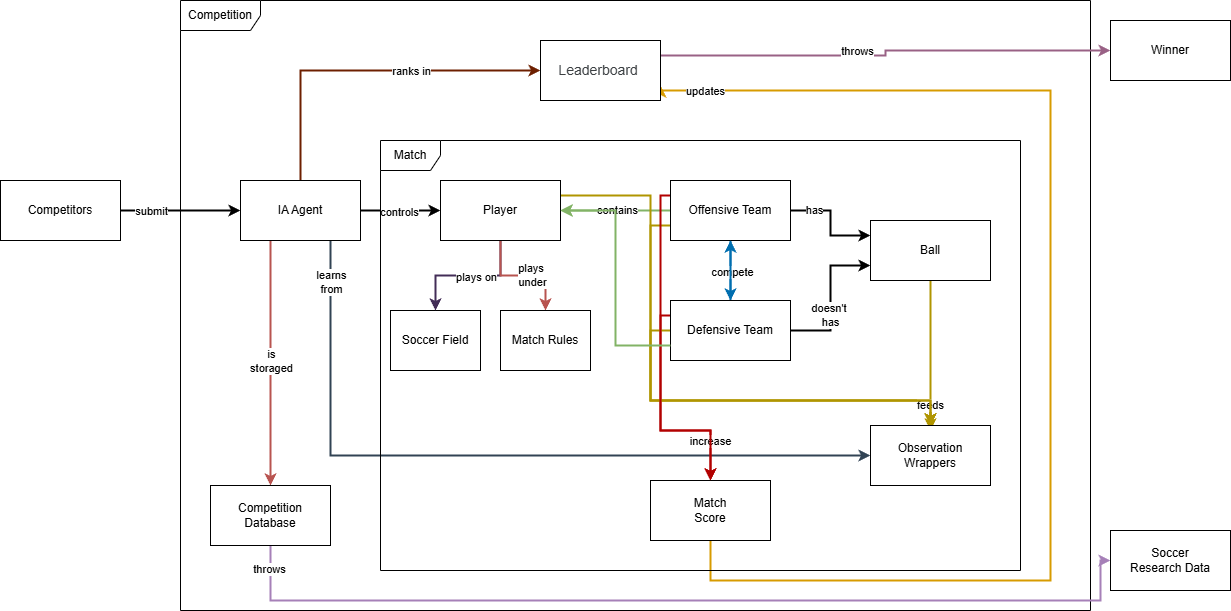
\includegraphics[width=\linewidth]{SystemMapping} 
    \caption{Competition as a system}
\end{figure}

\begin{enumerate}

    \item \textbf{Inputs:}
    \begin{itemize}
        \item Competitors who wants to participate in the competition.
    \end{itemize}

    \item \textbf{Elements of the system:}
    \begin{itemize}
        \item IA Agents submitted by competitors.
        \item Leaderboard that shows the top of the best IA Agents.
        \item Competition Database that stores all of the submissions made by the competitors.
        \item Match sub-system where the IA Agents compete with each other, composed of:
        \begin{itemize}
            \item Players.
            \item Soccer field.
            \item Match rules.
            \item Match score.
            \item Offensive team.
            \item Defensive team.
            \item Ball.
            \item Observation wrappers.
        \end{itemize}
    \end{itemize}

    \item \textbf{Outputs:}
    \begin{itemize}
        \item Winners of the competition.
        \item Soccer Research Data.
    \end{itemize}
\end{enumerate}

\subsection*{System Flow}
\begin{itemize}
\item The system recieves competitors who submit their IA Agent to participate, having two processes with it: the IA agent is stored on the Database of the competition, and the IA agent is tested in a match against itself to test if it works. The competitor can upload up to five agents per day.

\item If it doesn't pass the test, it will be returned as error. Otherwise, it is asignated with a base $\mu$ that represents the estimated skill of the agent, and a $\sigma$ that represents the uncertainty of that estimate, and will decrease everytime that the agent plays.

\item During the competition, the IA Agent with similar $\mu$ will play matches against each other. The winner increase its $\mu$, while the loser decrease it. If it's a draw, both $\mu$ will move closer towards their mean. Im any case, the leaderboard will be updated.

\item Starting a match, the simulation will assign randomly an IA agent per team. The teams are defined as left team, and right team, and unlike a real match of soccer, the teams will not switch sides in all the game.

\item During the match, Observation wrappers are generated and delivered to the IA Agents constantly, those contains general information about the match, like the match mode, position of all players, which player has the ball, etc. Everytime an observation wrappers is generated, the match moves forward one step. The duration of the match is 30000 steps in total. No aditional time can be added.

\item One IA Agent only controls one player of its team at time. If its team has the ball, the player will be the one with the ball. Otherwise, the player will be the closest to the ball. In every step IA Agents have to take decision based on the observation wrappers generated.

\item At the end of the competition, the competitors on the podium receive awards. While all the submits made during the competition are left to be used by the Google Research Football.
\end{itemize}

%Sensitivity
\graphicspath{{jorge/}}

\section{Sensitivity Analysis}
\section*{Sensitivity Analysis – Questions}

The objective of this analysis is to determine to what extent the system output, represented by the agent’s estimated performance ($\mu$), varies in response to changes in different inputs or configurations. The aim is to identify which factors have the greatest impact on the agent’s overall performance.

\begin{enumerate}
    \item \textbf{Type of data observation}
    \begin{itemize}
        \item Does the agent achieve better performance using observations in simple115\_v2, pixels, or raw format?
        \item The analysis will determine which type of input allows the model to better understand the environment.
    \end{itemize}

    \item \textbf{Actions used}
    \begin{itemize}
        \item Does using a reduced or extended set of actions significantly affect the agent's performance?
        \item It will be evaluated whether limiting or expanding the action options improves or worsens the agent's ability to make effective decisions.
    \end{itemize}

    \item \textbf{Training techniques}
    \begin{itemize}
        \item How sensitive is the performance ($\mu$) to changes in the training algorithm used?
        \item Comparison among methods such as PPO, A3C, and DQN to identify which achieves higher learning efficiency.
    \end{itemize}

    \item \textbf{Submission frequency and quantity}
    \begin{itemize}
        \item Does the frequency of agent submissions to the evaluation system influence performance?
        \item It will be investigated whether it's more effective to submit agents continuously or only when significant performance improvements are observed.
    \end{itemize}

    \item \textbf{Initial uncertainty ($\sigma$) and early learning}
    \begin{itemize}
        \item How beneficial is it to make multiple submissions during the early training stages compared to later stages?
        \item The goal is to understand whether an early approach helps reduce uncertainty and accelerate rating convergence.
    \end{itemize}

    \item \textbf{Agent policy change (exploration vs exploitation)}
    \begin{itemize}
        \item Do agents with more conservative strategies (exploitation) or more risk-taking strategies (exploration) achieve better results?
        \item This will analyze which approach tends to produce a higher $\mu$ value in the long term.
    \end{itemize}

    \item \textbf{Fatigue, roles, and red cards}
    \begin{itemize}
        \item How useful is it to include this type of additional context in the observations?
        \item It will be assessed whether considering these variables improves the agent’s decisions during gameplay.
    \end{itemize}

    \item \textbf{Goals and goal difference}
    \begin{itemize}
        \item How much does the number of goals or goal difference influence $\mu$ variation?
        \item The aim is to understand whether the final match score directly impacts the rating adjustment.
    \end{itemize}
\end{enumerate}

\section*{Sensitivity Analysis – Hypotheses}

\begin{enumerate}
    \item \textbf{Type of observation}
    \begin{itemize}
        \item Hypothesis: The way environment data is represented significantly affects the model's learning ability.
        \item Expected observation:
        \begin{itemize}
            \item simple115\_v2: allows faster and more efficient learning, with a higher initial $\mu$.
            \item raw: may lead to lower performance if not properly processed.
            \item pixels: requires more episodes and computational resources.
        \end{itemize}
        \item Sensitivity: High – Small changes in data representation can have a considerable impact on performance.
    \end{itemize}

    \item \textbf{Action set used}
    \begin{itemize}
        \item Hypothesis: A broader action set improves the agent’s adaptability in complex situations.
        \item Expected observation:
        \begin{itemize}
            \item Basic actions: quick but limited strategy.
            \item Extended actions: enables more strategic and versatile gameplay.
        \end{itemize}
        \item Sensitivity: Medium – Influences playing style and win probability.
    \end{itemize}

    \item \textbf{Training algorithm}
    \begin{itemize}
        \item Hypothesis: Some algorithms promote better exploration or converge more efficiently.
        \item Expected observation:
        \begin{itemize}
            \item PPO: stable and commonly used as a baseline.
            \item DQN: may struggle in continuous or complex environments.
            \item A3C: can be unstable, but trains policy and value function simultaneously.
        \end{itemize}
        \item Sensitivity: High – Directly affects how the agent learns from the environment.
    \end{itemize}

    \item \textbf{Submission frequency and quantity}
    \begin{itemize}
        \item Hypothesis: The submission strategy influences the agent’s visibility and optimization.
        \item Expected observation:
        \begin{itemize}
            \item Frequent submissions: can quickly rank the best agent.
            \item Selective and optimized submissions: avoid penalties from low-performing agents.
        \end{itemize}
        \item Sensitivity: Medium – Affects the amount and quality of feedback received to improve the model.
    \end{itemize}

    \item \textbf{Initial uncertainty ($\sigma$) and early learning}
    \begin{itemize}
        \item Hypothesis: Early stages are critical for establishing good positioning in the matchmaking system.
        \item Expected observation:
        \begin{itemize}
            \item Early submissions with good performance allow for rapid ranking.
            \item Late submissions may not reach optimal $\mu$ before the competition ends.
        \end{itemize}
        \item Sensitivity: High – Initial uncertainty ($\sigma$) and playtime strongly influence the rating.
    \end{itemize}

    \item \textbf{Play style (exploration vs. exploitation)}
    \begin{itemize}
        \item Hypothesis: Agents with high exploration may discover new strategies but compromise stability.
        \item Expected observation:
        \begin{itemize}
            \item High exploration: generates unexpected behaviors and potential tactical advantages.
            \item Low exploration: produces safer but more predictable behaviors.
        \end{itemize}
        \item Sensitivity: Medium – May be beneficial or detrimental depending on the tournament stage.
    \end{itemize}

    \item \textbf{Fatigue, cards, and player roles}
    \begin{itemize}
        \item Hypothesis: These factors may influence agent behavior, although their impact depends on the model and how the environment penalizes those conditions.
        \item Expected observation: They will only be useful if the agent is advanced enough to learn from these signals.
        \item Sensitivity: Medium – Add value in more complex and context-aware models.
    \end{itemize}

    \item \textbf{Goals and goal difference}
    \begin{itemize}
        \item Observation: The scoring system $\mu$ is based solely on the match result (win, draw, or loss), not on the number of goals.
        \item Sensitivity: Low – Winning by one or many goals does not affect $\mu$ update.
    \end{itemize}
\end{enumerate}

\section*{Visualization of Hypothetical Results (As part of the sensitivity analysis)}

A graph was created based on hypothetical results, constructed from reasonable assumptions consistent with the rating update system rules ($\mu$). This visualization does not use real data but reflects expected behaviors according to the dynamics of the competition environment.

\subsection*{Initial hypothesis:}
The analysis starts with a base value of $\mu$ = 600, common in matchmaking systems like TrueSkill or similar.

It evaluates how different configurations impact the evolution of the estimated rating during the first few days of the competition, within a possible range between 580 and 650.

This range is justified under the assumption that:
\begin{itemize}
    \item Agents are matched against opponents of similar level.
    \item $\mu$ updates after each match are moderate.
    \item In the early days, $\mu$ changes reflect the adaptation and initial learning process.
\end{itemize}

Variables analyzed:
\begin{itemize}
    \item Type of observation (simple115\_v2, raw, pixels)
    \item Training algorithm (PPO, A3C, DQN)
    \item Submission frequency (high vs. low frequency)
\end{itemize}

\begin{figure}
    \centering
    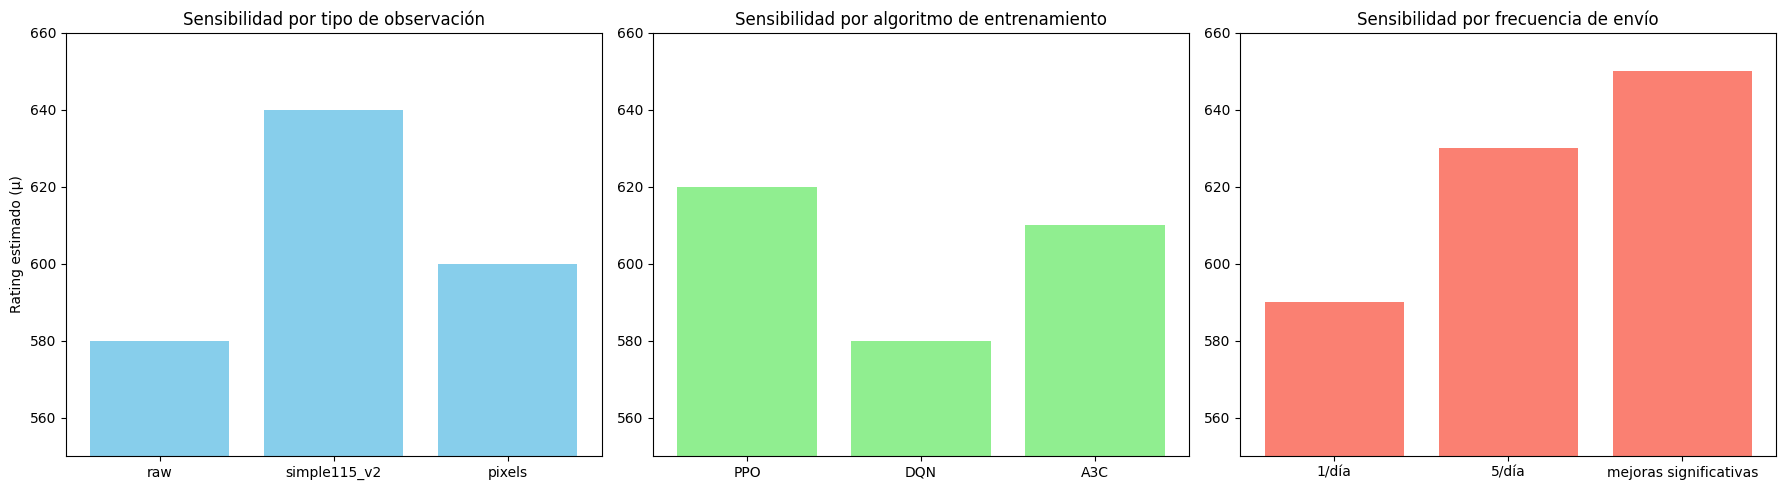
\includegraphics[width=\linewidth]{grafe} 
    \caption{Score Projection Charts}
    \label{fig:enter-label}
\end{figure}


\subsection*{Results Obtained (Graphs):}
The graph shows how, depending on the configuration:
\begin{itemize}
    \item Agents using simple115\_v2 tend to show a faster and more stable growth curve.
    \item Agents trained with PPO display a more consistent progression compared to A3C or DQN.
    \item Frequent submissions allow for quicker adjustments in the system, favoring continuous improvement in $\mu$, while sporadic submissions show less variation in the short term.
\end{itemize}

\section*{Conclusions}

\begin{tabular}{|l|l|l|}
\hline
Variables & Sensitivity & Importance \\
\hline
Training algorithm & High & Affects decisions → Wins → Affects $\mu$ \\
Type of observation & High & More information → Better performance \\
Submission frequency & High & Better $\mu$ estimates and feedback \\
Action set & Medium & Influences the agent’s tactical execution \\
Fatigue, Roles, Cards & Medium & Useful in specific moments \\
Play style & Medium & Specific, infrequent cases \\
Goals/Goal difference & Low & Does not affect $\mu$ updates \\
\hline
\end{tabular}
 

%Chaos Theory
\section{Chaos Theory in Football}

A sport like football is largely subject to chance and, therefore, to chaos. In it, a single individual action can completely change the course of the match—such as a foul that leads to a player's expulsion, a counterattack that occurs independently of the game's context, a mistake by a player or even the referee. Even factors like the field and the weather are fundamental elements that do not depend on the players themselves and can seriously affect the outcome of the match.

All these types of situations are quite difficult to transfer into simulation environments, as these are usually carried out under perfect conditions. If such cases were incorporated into simulations, the results could be more efficient and realistic.

In these environments, artificial intelligence can misinterpret data due to random factors. An AI agent might develop a very effective strategy that allows it to control the match for most of the time, but due to one of these isolated events, it could interpret its strategy as ineffective.

Factors such as rebounds strongly influence the outcome of matches, and they are unpredictable, generating dangerous plays that could impact the final result.





%Conclusion
\section{Conclusion}

From a system's point of view, the AI Football Competition illustrates a complex interplay between inputs (agent submissions and parameters), processing (match simulations and learning methods), and outputs (performance grades and research outcomes). The design of the system facilitates scalable evaluation via auto-matching, whereby agents of similar skill levels compete in sandboxed environments. This setup guarantees scalability and perpetual benchmarking, with participants able to tune their models according to observations from the leaderboard.

The system also has some contemporary limitations since it operates in a closed-loop fashion. The simulation provides structured observations, including the position of the players, where the ball travels, and game state. Still, it operates within a structured environment, discluding real-life challenges such as environmental conditions and human unpredictability. The structured action space prevents unusual behaviors as agents cannot implement unorthodox strategies outside designated actions. Furthermore, while the rating system is effective for establishing rankings, it may inadvertently encourage conservative playing styles that exploit limitations in simulation rather than showcasing genuine football skills.

Future improvements could include adding complexity by adding changing factors, like changing pitch conditions and referee mistakes, and adaptive rules that change depending on the agents' performance. A feedback loop based on real match data could also help connect the simulation back to reality. Ultimately, the strength of the competition is in the pipelined evaluation framework, but its long-term sustainability is in accepting the messy, nonlinear systems that characterize real football where agents have to deal not only with adversaries, but with the intrinsic uncertainty of the game itself.
\begin{thebibliography}{9}

    \bibitem{kaggle_football}
    Google. \emph{Google Research Football with Kaggle}, 2020.\\
    \url{https://www.kaggle.com/competitions/google-football/overview}.\\
    Accessed: 2025-04-04.
    
    \bibitem{rules_of_football}
    Rules of Sport. \emph{Football Rules}.\\
    \url{https://www.rulesofsport.com/sports/football.html}.\\
    Accessed: 2025-04-04.
    
    \bibitem{kaggle_football_json}
    Kaggle. \emph{Football Environment JSON Config}.\\
    \url{https://github.com/Kaggle/kaggle-environments/blob/master/kaggle_environments/envs/football/football.json}.\\
    Accessed: 2025-04-04.
    
    \bibitem{kaggle_football_py}
    Kaggle. \emph{Football Environment Python File}.\\
    \url{https://github.com/Kaggle/kaggle-environments/blob/master/kaggle_environments/envs/football/football.py}.\\
    Accessed: 2025-04-04.
    
    \bibitem{google_research_football}
    Google Research. \emph{Google Research Football GitHub Repository}.\\
    \url{https://github.com/google-research/football/}.\\
    Accessed: 2025-04-04.
    
    \bibitem{google_research_observation}
    Google Research. \emph{Google Football Observation Documentation}.\\
    \url{https://github.com/google-research/football/blob/master/gfootball/doc/observation.md#raw-observations}.\\
    Accessed: 2025-04-04.
    
    \end{thebibliography}
    
\end{document}